\section{Recommendation Systems (Öneri Sistemleri)}
Öneri sistemleri (recommendation systems), kullanıcılara ürünler, içerik veya hizmetler hakkında kişiselleştirilmiş öneriler sunan bir tür yapay zeka uygulamasıdır. Bu sistemler, genellikle büyük veri kümelerini analiz ederek ve kullanıcıların geçmiş etkileşimleri veya tercihleri gibi bilgileri kullanarak, kullanıcıların ilgisini çekebilecek öğeleri tahmin etmeye çalışırlar. Öneri sistemleri, e-ticaret siteleri, video akış platformları, müzik akış servisleri, haber siteleri ve daha pek çok alanda kullanılır. ikiye ayrılır:

\begin{itemize}
    \item İçerik Tabanlı (Content-Based) Öneri Sistemleri
    \item İşbirliği Tabanlı (Collaborative) Öneri Sistemleri
\end{itemize}

\begin{figure}[h]
    \centering
    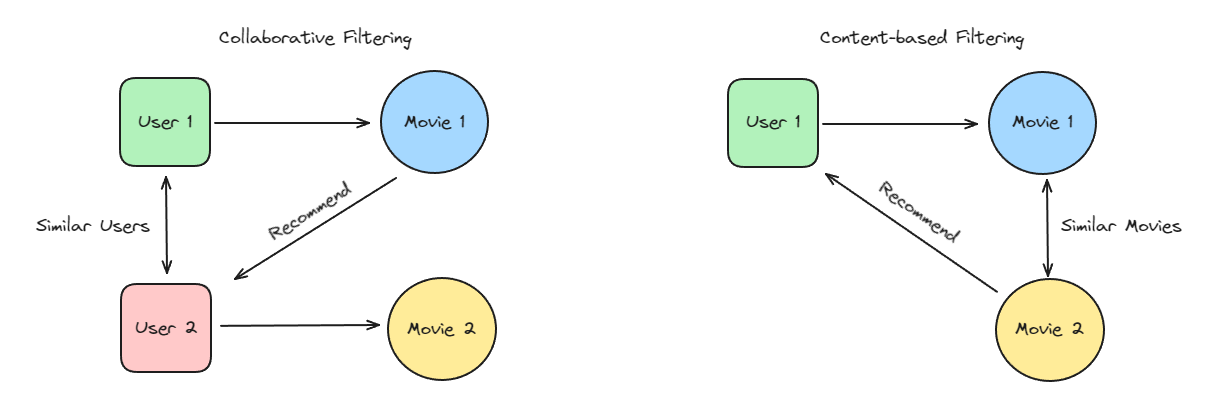
\includegraphics[width=1\textwidth]{images/filtering_types.png}
    \caption{Öneri sistemleri türleri.}
    \label{fig:enter-label}
\end{figure}

\subsection{Content-Based Filtering}
İçerik tabanlı öneri sistemleri, kullanıcılara belirli öğeleri veya içerikleri kişiselleştirilmiş önerilerle sunan bir tür yapay zeka uygulamasıdır. Bu sistemler, kullanıcıların veya öğelerin içerik özelliklerini analiz ederek çalışırlar. İçerik tabanlı öneri sistemleri, bir kullanıcının geçmiş tercihleri ve incelemeleri gibi verileri kullanarak, bu kullanıcının ilgisini çekebilecek benzer içerikleri önerir.Content-based öneri sistemlerinde kullanılan benzerlik hesaplama yöntemleri, kullanıcı profili ile içerik özellikleri arasındaki benzerliği değerlendirmek için kullanılır.\\

\textbf{Kosinüs Benzerliği (Cosine Similarity):} Vektörler arasındaki açıyı ölçerek benzerliği hesaplar. Kullanıcı profil vektörü ile her öğe arasındaki kosinüs benzerliği hesaplanır.

\begin{lstlisting}[language=Python]
import numpy as np
from sklearn.metrics.pairwise import cosine_similarity

# Ozellik vektorleri: Her bir satir bir filmi temsil eder.
# Her bir sutun bir turu temsil eder. Ornegin, 1. sutun "Aksiyon", 2. sutun "Komedi" vb.
# Ornek ozellik vektorleri sadece temsil amaclidir.
features = np.array([
    [1, 0, 1, 0, 1],  # Film 1: Aksiyon ve Bilim Kurgu
    [0, 1, 0, 1, 0],  # Film 2: Komedi
    [1, 0, 0, 0, 1],  # Film 3: Aksiyon ve Korku
    [0, 0, 0, 1, 1]   # Film 4: Korku
])

# Kullanici profil vektoru: Kullanicinin tur tercihlerini temsil eder.
user_profile = np.array([1, 1, 0, 0, 0])  # Kullanici Aksiyon ve Komedi filmlerini sever.

# Cosine similarity hesaplama
similarities = cosine_similarity([user_profile], features)

# Benzerlik skorlari ve onerilen filmler
similarities = similarities[0]  # Tek bir kullanicinin benzerlik skorlari
recommended_movies = np.argsort(similarities)[::-1]  # Benzerlik sirasina gore filmleri sirala

print("Benzerlik Skorlari: ", similarities) # Benzerlik Skorlari:  [0.40824829, 0.5, 0.5, 0.]
print("Onerilen Filmler (Sirasiyla): ", recommended_movies) # Onerilen Filmler (Sirasiyla):  [2 1 0 3]
# Film 3, Film 2, Film 1, Film 4
\end{lstlisting}

\textbf{Jaccard Benzerliği (Jaccard Similarity):} İki kümenin kesişimini birleşimine bölen bir oranı ifade eder. Özelliklerin varlığı veya yokluğuyla ilgili olduğu için sıklıkla kategorik veriler üzerinde kullanılır.

\begin{lstlisting}[language=Python]
import numpy as np

# Film turlerini temsil eden ozellik vektorleri (ornek veri)
# Her satir bir filmi temsil eder, her sutun bir turu temsil eder.
# Ornegin, 1. sutun "Aksiyon", 2. sutun "Komedi" vb.
features = np.array([
    [1, 0, 1, 0, 0],  # Film 1: Aksiyon ve Bilim Kurgu
    [0, 1, 0, 1, 0],  # Film 2: Komedi ve Romantik
    [1, 0, 0, 0, 1],  # Film 3: Aksiyon ve Korku
    [0, 0, 0, 1, 1]   # Film 4: Korku
])

# Kullanicinin tur tercihlerini temsil eden ozellik vektoru
user_profile = np.array([1, 1, 0, 0, 0])  # Kullanici Aksiyon ve Komedi filmlerini sever.

def jaccard_similarity(a, b):
    intersection = np.logical_and(a, b)
    union = np.logical_or(a, b)
    return np.sum(intersection) / np.sum(union)

# Jaccard benzerligi hesaplama
similarities = [jaccard_similarity(user_profile, film_features) for film_features in features]

# Benzerlik skorlari ve onerilen filmler
recommended_movies = np.argsort(similarities)[::-1]  # Benzerlik sirasina gore filmleri sirala

print("Benzerlik Skorlari: ", similarities) # [0.33, 0.33, 0.33, 0.0]
print("Onerilen Filmler (Sirasiyla): ", recommended_movies) # Onerilen Filmler (Sirasiyla):  [2 1 0 3]
\end{lstlisting}

\textbf{Öklidyen Uzaklığı (Euclidean Distance):} İki nokta arasındaki doğrusal uzaklığı hesaplar.

\begin{lstlisting}[language=Python]
import numpy as np

# Ozellik vektorleri: Her bir satir bir filmi temsil eder.
# Her bir sutun bir ozelligi temsil eder.
features = np.array([
    [2.5, 1.0, 3.0],  # Film 1
    [1.5, 2.5, 0.5],  # Film 2
    [2.0, 3.5, 2.5],  # Film 3
    [0.5, 1.5, 3.0]   # Film 4
])

# Kullanici profil vektoru: Kullanicinin tercih ettigi ozelliklerin agirliklarini icerir.
user_profile = np.array([3.0, 1.5, 2.0])

def euclidean_distance(a, b):
    return np.linalg.norm(a - b)

# Oklidyen mesafe hesaplama
distances = [euclidean_distance(user_profile, film_features) for film_features in features]

# Uzaklik skorlari ve onerilen filmler
recommended_movies = np.argsort(distances)  # Uzaklik sirasina gore filmleri sirala

print("Uzaklik Skorlari: ", distances) # Uzaklik Skorlari:  [1.22, 2.34, 2.29, 2.69]
print("Onerilen Filmler (Sirasiyla): ", recommended_movies) # Onerilen Filmler (Sirasiyla):  [0 2 1 3]
\end{lstlisting}

\subsection{Collaborative Filtering}
Collaborative Filtering (İşbirlikçi Filtreleme), kullanıcıların veya öğelerin geçmiş etkileşimlerini temel alarak kişiselleştirilmiş öneriler sunan bir öneri sistemlerinin bir türüdür. Bu yöntem, kullanıcıların benzer tercihleri olan diğer kullanıcıları veya öğeleri bulur ve bu benzerliklere dayanarak önerilerde bulunur.

\begin{itemize}
    \item \textbf{Benzer Kullanıcılar (User-Based Collaborative Filtering):} Bu yöntem, kullanıcıların benzer tercihlere sahip olan diğer kullanıcıları bulur. Örneğin, kullanıcı A ve kullanıcı B benzer filmleri beğeniyorsa, kullanıcı A'nın beğendiği ancak kullanıcı B'nin görmediği bir filmi kullanıcı B'ye önerir. Benzer kullanıcıları bulmak için yaygın olarak kullanılan ölçümler arasında kosinüs benzerliği veya Pearson korelasyon katsayısı bulunur.
    \item \textbf{Benzer Öğeler (Item-Based Collaborative Filtering):} Bu yöntem, benzer özelliklere sahip olan öğeleri bulur ve kullanıcıların geçmiş etkileşimleri temel alarak benzer öğeleri önerir. Örneğin, bir kullanıcı film A'nın benzer türdeki film B'yi beğendiyse, film B'yi kullanıcıya önerir. Benzer öğeleri bulmak için kullanılan ölçümler arasında cosine similarity veya Jaccard similarity gibi metrikler bulunur.
\end{itemize}

İşbirlikçi Filtreleme yöntemleri, genellikle "user-item matrix" olarak adlandırılan bir veri matrisini kullanır. Bu matris, kullanıcıların öğelerle olan etkileşimlerini veya derecelendirmelerini içerir. Boş değerler, kullanıcının belirli bir öğe ile etkileşimde bulunmadığını veya öğeyi derecelendirmediğini gösterir.

\newpage